Release flow is a set of steps to perform to release upcoming version of software product.
Main aim of this document is to present simple and working model of software release
using Semantic versioning~\cite{SemanticVersioning}, \texttt{Azure pipelines}
and \texttt{Mainline} development~\cite{MainlineDevelopment}.
Mainline development is also known as GitHub flow.
Current document is motivated by Microsoft's
\textit{Adopt a GIT branching strategy} available at~\cite{AdoptGitStrategy}.
The picture below shows the main idea of GitHub flow
\begin{figure}[H]
    \centering
    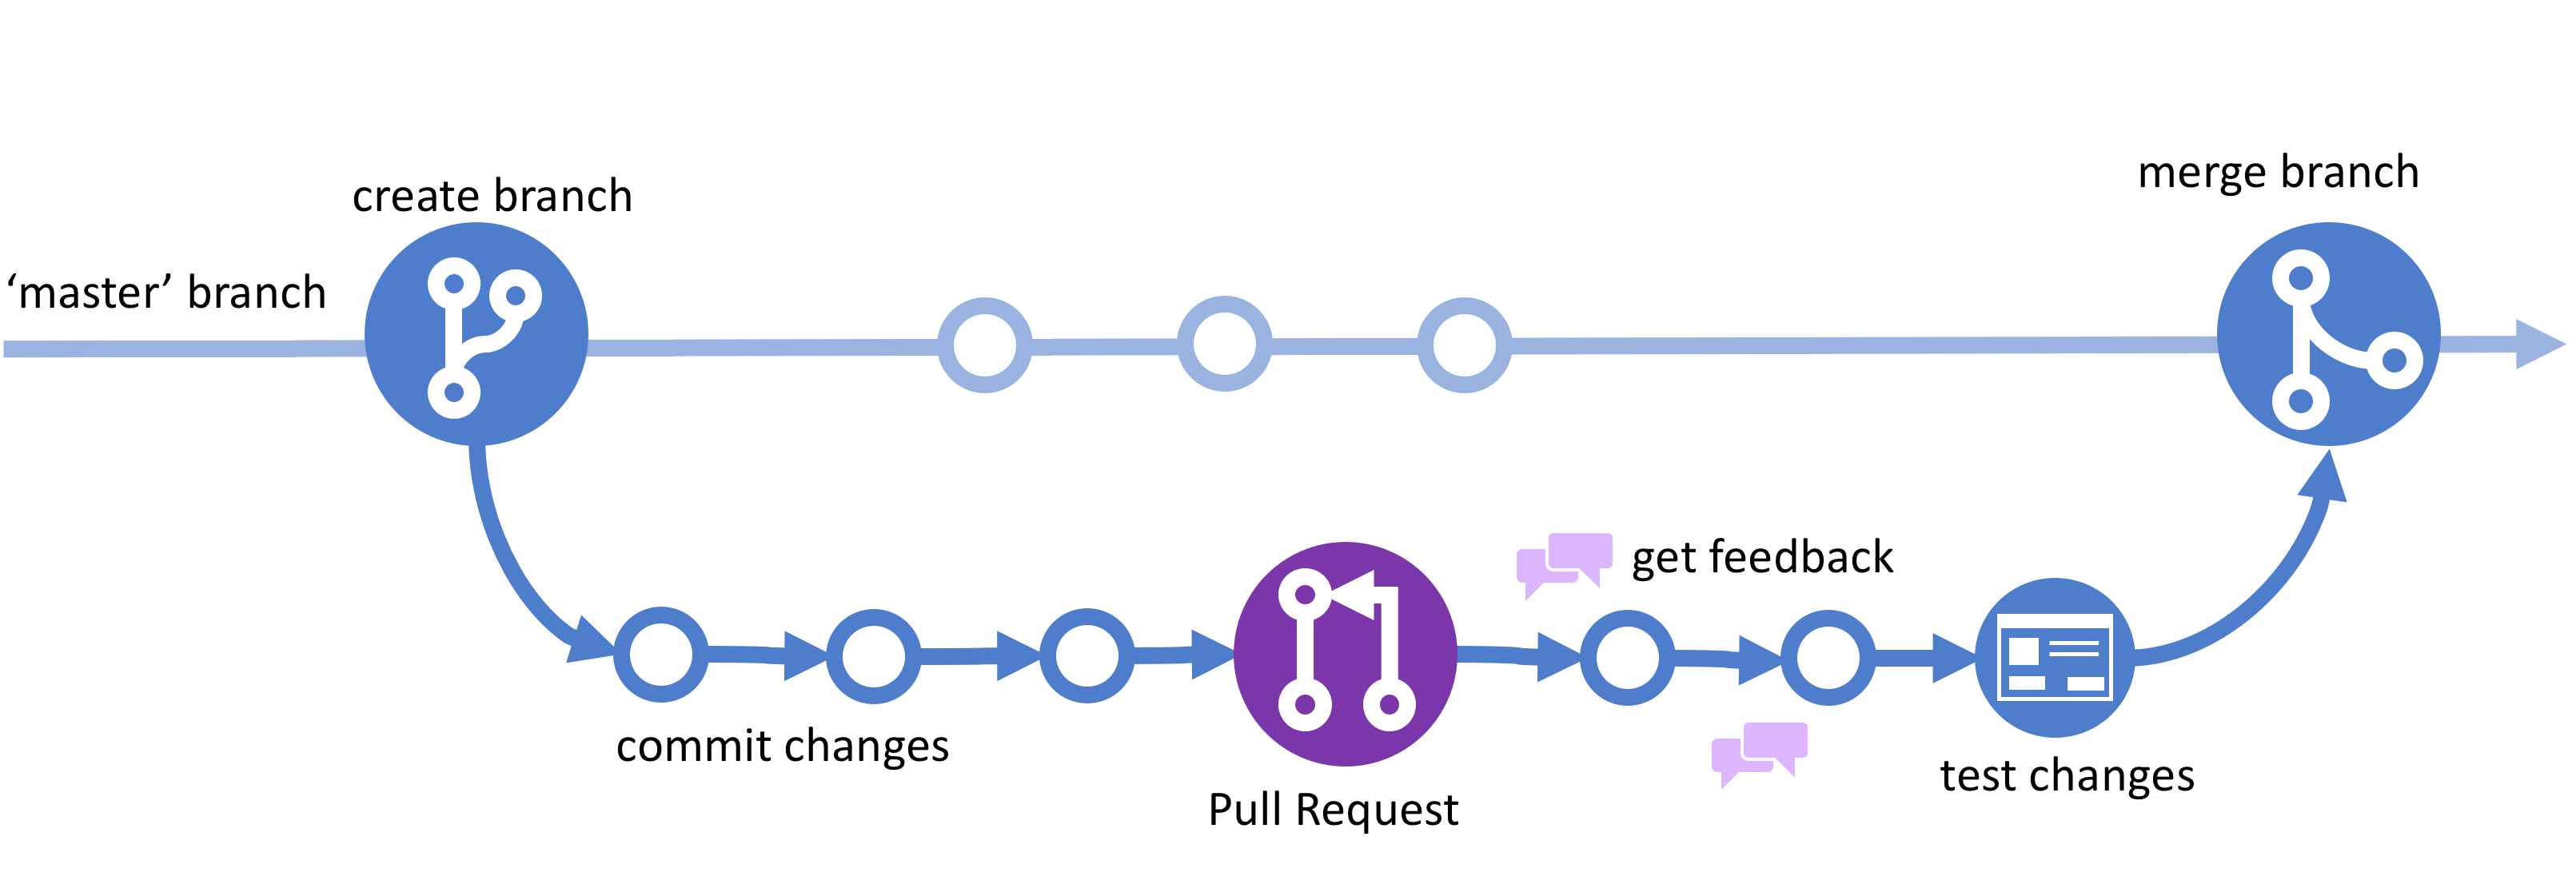
\includegraphics[width=1\textwidth]{img/GitHub_Flow}
    ~\caption{GitHub Flow diagram.}\label{fig:github-flow}
\end{figure}

\begin{itemize}
    \item \textbf{Master} -- branch that contains tested, validated and verified code, ready to be released and deployed to production.
    \item \textbf{Feature} -- branch that contains implementation of a new feature according to sprint plan.
    The \texttt{feature} branch is based onto \texttt{master}.
    \item \textbf{Bugfix} -- branch that contains non-critical bug fix.
    The \texttt{bugfix} branch is based onto \texttt{master}, and merged back to \texttt{master} after fix is done.
    \item \textbf{Release/v*} -- branch that contains upcoming release state of software product, serves to keep small changes
    and updates to \texttt{CHANGELOG} file.
    The \texttt{Release/v*} branch is based onto \texttt{master}.
    The \texttt{Release/v*} branch is considered to be long-living branch, it should not be deleted after code is deployed to production.
    After release is completed it is merged back to \texttt{master}.
    \item \textbf{Hotfix} -- branch that contains critical bug fix.
    It is used to patch production environment and must be released as quick as possible.
    The \texttt{hotfix} branch is based onto the latest released \texttt{Release/v*} branch.
    After hotfix is released it is merged back to its base \texttt{Release/v*} and Cherry-picked~\cite{CherryPick}
    by \texttt{master}.
\end{itemize}

\subsection{Release process}\label{subsec:release-process}
Having all above, assume we have initial semantic version of our application as \texttt{v1.0.0},
so that we must release upcoming version.
The version \texttt{1.0.0} has been tested by QA team, so that release was approved by whole team.
General release steps to perform are following
\begin{enumerate}
    \item \textbf{Code phase.}
    Software engineer creates pull request from recent \texttt{feature} branch to \texttt{master} branch,
    this pull request triggers Continuous Integration (CI) to start, CI runs tests, code quality checks etc.,
    but deployment is not started yet, only CI\@.
    \item \textbf{Code phase.}
    After all CI checks passed, pull request reviewed by team and every comment from code review is fixed --
    the \texttt{feature} branch is ready to be merged into \texttt{master} branch.
    No CI/CD pipeline triggered by the merge.
    \item \textbf{Code phase.}
    Next, release engineer reviews software product changes documenting them in \texttt{CHANGELOG} file.
    Release engineer decides on the next Semantic Version~\cite{SemanticVersioning} increment.
    For example, software product has breaking changes,
    then release engineer decides to increment the major part of semantic version, so that \texttt{v0.1.1 -> v1.0.0}
    \item \textbf{Code phase.}
    Release engineer creates new release as follows
    \begin{itemize}
        \item Checkout to release branch: \texttt{git checkout -b release/v1.0.0}
        \item Adding minor changes and \texttt{CHANGELOG} file update
        \item Push release branch to remote: \texttt{git push origin release/v1.0.0}
        \item Create tag: \texttt{git tag -a v1.0.0 -m "Release v1.0.0"}
        \item Push tag: \texttt{git push origin v1.0.0}
    \end{itemize}
    \item \textbf{Build phase.}
    When new \texttt{TAG} is pushed to the remote repository, the build pipeline is being triggered~\cite{AzurePipelinesTriggers},
    initializing the build phase of DevOps cycle.
    Therefore, the code is being built, tested and specific artifacts are being created and published.
    \item \textbf{Release phase.} Release engineer validates the build artifacts,
    underlying infrastructure and deployment automations, ensuring smooth and reliable upcoming deployment.
    \item \textbf{Deploy phase.}
    There are a few deployments scheduled including the environments \texttt{DEV}, \texttt{QA}, \texttt{UAT}.
    Deployments to \texttt{QA} and \texttt{UAT} environments are to be approved by designated personnel,
    meanwhile \texttt{DEV} environment to be deployed automatically.
    \item Finally, the \texttt{Release/v*} branch is merged back to \texttt{master} after deployment is complete.
\end{enumerate}
Entire release process is shown on the picture below
\begin{figure}[H]
    \centering
    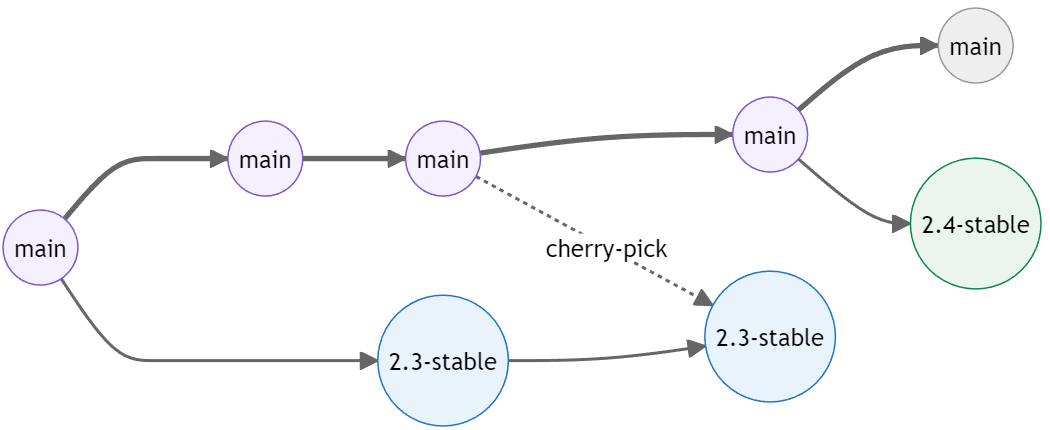
\includegraphics[width=1\textwidth]{img/GitLab_Flow}
    ~\caption{GitLab Flow diagram~\cite{GitLabFlow}.}\label{fig:gitlab-flow}
\end{figure}



\subsection{Hotfix strategy}\label{subsec:hotfix-strategy}
Assume that our current released version of software product is \texttt{v0.2.0} and there is a critical bug appears.
In order to release a hotfix the following set of steps to be executed:
\begin{enumerate}
    \item Hotfix to be assigned to a software engineer.
    \item Software engineer fixes critical bug and creates a pull request: \texttt{hotfix/id -> master}.
    Yes, pull request is done to the \texttt{master} branch.
    \item Pull request \texttt{hotfix/id -> master} is reviewed by team and merged.
    \item Release engineer cherry-picks~\cite{CherryPick} recently merged hotfix from the \texttt{master} branch
    to the \texttt{release/v0.2.0} branch.
    Note that branch \texttt{release/v0.2.0} is long-living and kept minimum until next release.
    \item Release engineer increments patch part of semantic version, e.g \texttt{v0.2.0 -> v0.2.1}.
    \item Release engineer creates and pushes new tag \texttt{v0.2.1}.
    \item Hotfix deployment process is started after new tag is pushed.
\end{enumerate}

